\include{__header__}

\begin{document}
\paragraph{О-02}
Общая схема наблюдения интерференции. Когерентные источники. Временная когерентность электромагнитных волн. Длина когерентности. Связь временной когерентности с степенью монохроматичности. Пространственная когерентность электромагнитных волн. Радиус когерентности. Интерференция в тонких пленках.\\

\begin{definition}
Интерференцией называется взаимное увеличение(уменьшение) результирующей амплитуды двух или нескольких волн при их наложении друг на друга.
\end{definition}

\begin{definition}
Два световых источника, способных создать интерференционную картину называются когерентными.
\end{definition}

\begin{theorem}[Условие когерентности источников]
Два источника света являются когерентными, если
\begin{enumerate}
\item они испускают свет одинаковой частоты;
\item угол между плоскостями колебаний световых векторов
\footnote{
	векторов напряженности электрических полей электромагнитных волн.
}
достаточно мал.
\item разность фаз в точке наблюдения изменяется незначительно (менее чем на $\pi$) за время усреднения прибора наблюдения.
\end{enumerate}
\end{theorem}
\begin{proof}
Рассмотрим две волны одной частоты $\omega$ (первое условие) со световыми векторами:
\begin{gather*}
\vec{E}_1 = \vec{E}_{10}e^{-i(\omega t - \varphi_1)},\qquad
\vec{E}_2 = \vec{E}_{20}e^{-i(\omega t - \varphi_2)},
\end{gather*}
где $\vec{E}_{10}, \vec{E}_{20}$ - амплитуды, $\varphi_1, \varphi_2$ - начальные фазы.
По принципу суперпозиции найдем световой вектор результирующего колебания:
$$
\vec{E} = \left(\vec{E}_{10}e^{i\varphi_1}+\vec{E}_{20}e^{i\varphi_2}\right)e^{-i\omega t} =
\vec{E}_0 e^{-i \omega t}
$$
отыщем интенсивность $I$ как квадрат модуля светового вектора:
\begin{flalign}
\label{o-02-intense}
\begin{split}
E^2 &= \left(\vec{E}_{10}e^{i\varphi_1}+\vec{E}_{20}e^{i\varphi_2}\right)
       \left(\vec{E}_{10}e^{-i\varphi_1}+\vec{E}_{20}e^{-i\varphi_2}\right) =\\
    &= E^2_{10} + E^2_{20} + 2(\vec{E}_{10}, \vec{E}_{20})\cos(\varphi_2 - \varphi_1),
\end{split}
\end{flalign}

определим $\angle(\vec{E}_{10},\vec{E}_20) = \alpha$, тогда (\ref{o-02-intense}) примет вид:
\begin{flalign}
\label{o-02-alpha}
I = I_1 + I_2 + 2\sqrt{I_1 I_2}\cos(\alpha)\langle\cos(\Delta \varphi)\rangle,
\end{flalign}
где $\langle\cos(\Delta \varphi)\rangle$ - разность фаз, усредненная по времени наблюдения прибора
\footnote{
	время отклика прибора измерения, которое, хоть и достаточно мало (для глаза это $0.1~\text{c.}$), но на порядки больше периода колебаний световой волны ($\sim 10^{-15}~\text{c.}$)
}
, $I_1 = E_1^2$, $I_2 = E_2^2$.

Из второго условия положим $\cos(\alpha)\approx 1$, тогда (\ref{o-02-alpha}) примет вид:
\begin{gather}
\label{o-02-mainint}
I = I_1 + I_2 + 2\sqrt{I_1 I_2}\langle\cos(\Delta \varphi)\rangle
\end{gather}
где $2\sqrt{I_1 I_2}\langle\cos(\Delta \varphi)\rangle$ называется интерференционным членом.

Заметим, что если разность фаз волн изменяются более чем на $\pi$ за время усреднения, то интерференционный член исчезает, и интерференция не наблюдается, иначе происходят периодические изменения интенсивности, т.е. наблюдается интерференция.
\end{proof}

Тогда из определения фазы волны: $\varphi = \vec{k}\vec{x}$ ($\vec{k}$ - волновой вектор, $\vec{x}$ - радиус-вектор) или вдоль светового луча: $\varphi = kl$, причем $l$ - путь, пройденный в среде, и для разных сред:
$$
\varphi = \sum_{i=1}^{N}k_i l_i = k\sum_{i=1}^{N}n_i l_i = kL,
$$
где $k$ - волновое число в вакууме, $n_i$ - коэффициент преломления среды, $L$ называется оптической длиной пути.
Тогда для двух волн одной частоты с фазами $\varphi_1$ и $\varphi_2$ разность их фаз примет вид:
\begin{gather}
\label{o-02-phasediff}
\Delta \varphi = k(L_2 - L_1) = k \Delta =
(k = \frac{2\pi}{\lambda}) =
\frac{2\pi}{\lambda}\Delta,
\end{gather}
где $\Delta$ называется оптической разностью хода. 

\begin{wrapfigure}[14]{R}{0.4\linewidth}
	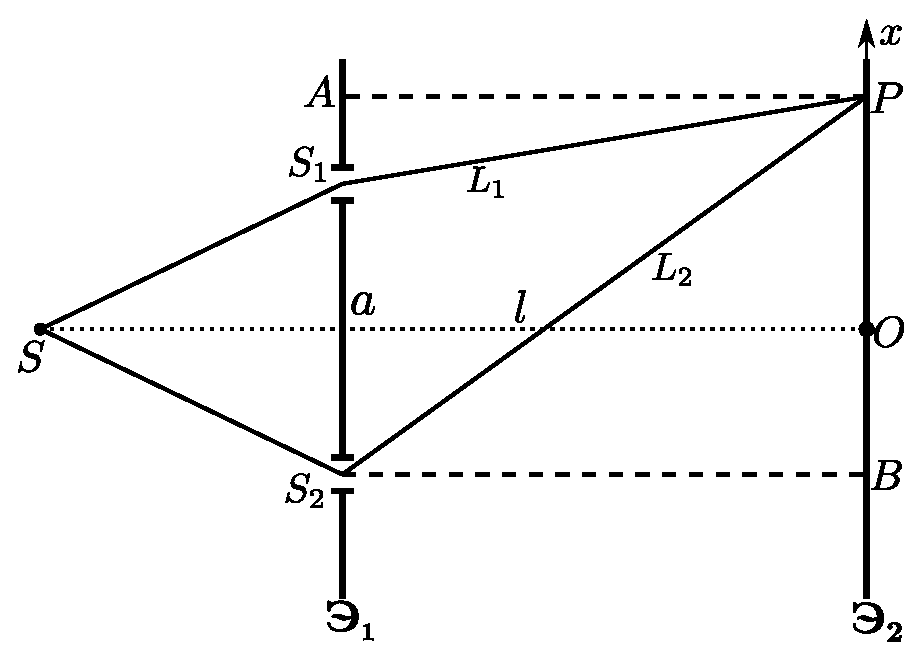
\includegraphics[width=1\linewidth]{img/o-02}{}
	\caption{Общая схема наблюдения интерференции}
	\label{o-02-scheme}
\end{wrapfigure}
 
\textbf{Общая схема наблюдения интерференции.}
Световые лучи от источника $S$ проходят через две щели на экране $\text{Э}_1$, образуя два источника $S_1$ и $S_2$. Лучи от этих источников попадают на экран $\text{Э}_2$, на котором наблюдается интерференционная картина в виде плавно переходящих друг в друга светлых полос, перпендикулярных плоскости рисунка.

Отыщем вид (\ref{o-02-mainint}) для этой схемы, для этого найдем $\Delta = L_2 - L_1$. Из
$\triangle S_1AP$ и $\triangle S_2BP$ отыщем $L_1$ и $L_2$ (см. Рис. \ref{o-02-scheme}):
$$
L_1 = \sqrt{l^2 + \left(x-\frac{a}{2}\right)^2}, \qquad
L_2 = \sqrt{l^2 + \left(x+\frac{a}{2}\right)^2},
$$
положим $l \gg a, \ l \gg |x|$ и воспользуемся теоремой Тейлора для $L_1$ и $L_2$:
\begin{gather*}
L_1 \approx l + \frac{\left(x-a/2\right)^2}{2l}, \qquad
L_2 \approx l + \frac{\left(x+a/2\right)^2}{2l},
\end{gather*}
тогда
\begin{gather}
\label{o-02-schemediff}
\displaystyle \Delta = L_2 - L_1 = \frac{xa}{l}
\end{gather}
Запишем формулу для интенсивности (\ref{o-02-mainint}) с учетом (\ref{o-02-schemediff}):
\begin{gather*}
I = I_1 + I_2 + 2\sqrt{I_1 I_2}\cos\left(\frac{2\pi}{\lambda}\Delta\right) =
    I_1 + I_2 + 2\sqrt{I_1 I_2}\cos\left(\frac{\pi x a}{\lambda l}\right),
\end{gather*}
для $I_1 = I_2 = I_0$:
\begin{gather}
\label{o-02-intensesch}
I = 2I_0\left(1 + \cos\left(\frac{2\pi}{\lambda}\Delta\right)\right) =
4I_0\cos^2\left(\frac{\pi xa}{\lambda l}\right),
\end{gather}

\begin{wrapfigure}[6]{R}{0.4\linewidth}
	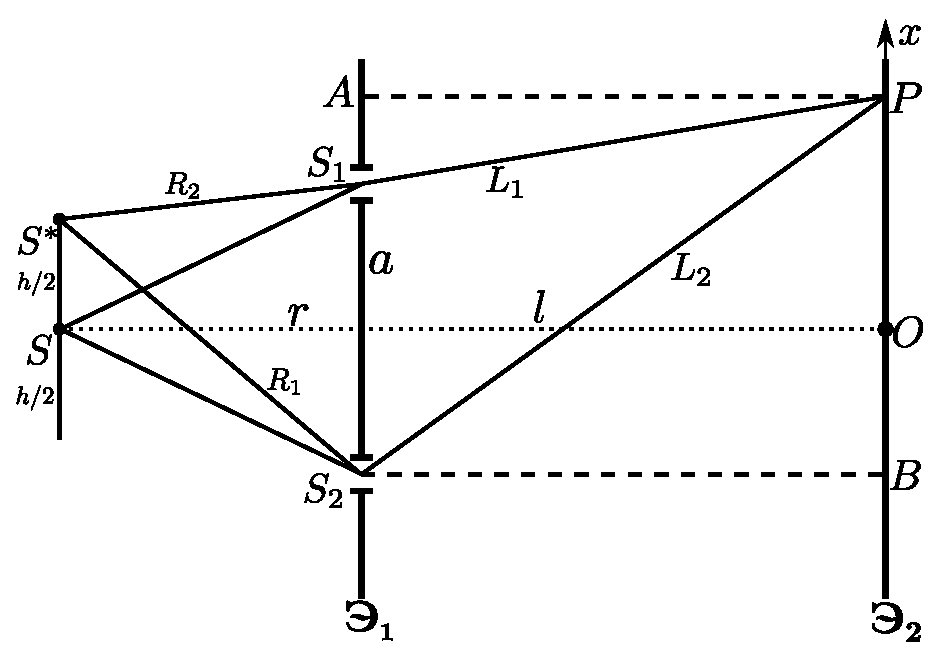
\includegraphics[width=1\linewidth]{img/o-02_1}{}
	\caption{К пространственной когерентности}
	\label{o-02-prostra}
\end{wrapfigure}

\textbf{Пространственная когерентность.}
Рассмотрим общую схему интерференции с новым источником $S^*$, смещенными на $h/2$ относительно старого $S$ (см. Рис. \ref{o-02-prostra}). Положим, что для расстояния до экрана $\text{Э}_1$ $r$ выполняется: $a\ll r, h\ll r$. Тогда аналогично предыдущему пункту получим добавочную разность хода до экрана $\text{Э}_1$: $\Delta^* = \frac{ha}{2r}$. Добавочная разность фаз согласно (\ref{o-02-phasediff}) примет вид $\displaystyle\psi = \frac{2\pi}{\lambda}\Delta^*$, тогда перепишем (\ref{o-02-intensesch}):
\begin{gather}
\label{o-02-intensetwo}
I = 2I_0\left(1+\cos\left(\psi + \frac{2\pi}{\lambda}\Delta\right)\right),
\end{gather}

Теперь положим источник отрезком $[-h/2, h/2]$ и отыщем интенсивность, для этого усредним (\ref{o-02-intensetwo}) по фазе $\psi$ от $-\Delta\psi/2$ (нижний конец) до $\Delta\psi/2$ (верхний).
\begin{flalign*}
\begin{split}
\langle I \rangle &=
\frac{2I_0}{\Delta\psi}
\int\limits_{-\Delta\psi/2}^{\Delta\psi/2}
\left(
	1 + \cos\left(\psi + \frac{2\pi}{\lambda}\Delta\right)
\right)d\psi = \\
&= 2I_0\left(
	1 + \frac{2\sin(\Delta\psi/2)}{\Delta\psi}\cos\left(\frac{2\pi}{\lambda}\Delta\right)
\right) = \\
&= 2I_0\left(
1 + G(\Delta\psi)\cos\left(\frac{2\pi}{\lambda}\Delta\right)
\right),
\end{split}
\end{flalign*}
при $\Delta\psi \rightarrow 0$ $G(\Delta\psi) \rightarrow 1$ (первый замечательный предел), т.е получаем формулу (\ref{o-02-intensesch}) для точечного источника.
Отыщем значение $\Delta\psi$ при котором интерференционная картина пропадает. Это, очевидно, происходит при минимальном $\Delta\psi$ таком, что $G(\Delta\psi) = 0$. Т.е
\begin{flalign*}
\begin{split}
&\frac{\Delta\psi}{2} = \pi
\Rightarrow (\Delta\psi = \frac{2\pi}{\lambda}\frac{ha}{r}) \\ \Rightarrow
&\frac{\pi ha}{\lambda r} = \pi \Rightarrow a = \frac{\lambda r}{h},
\end{split}
\end{flalign*}
тогда для наблюдения пространственной интерференции должно выполняться условие 
$$
a < \frac{\lambda r}{h} = \rho_\text{ког}.
$$

\begin{definition}
Величину $\displaystyle \rho_\text{ког} = \frac{\lambda r}{h}$ называют радиусом когерентности.
\end{definition}

\textbf{Временная когерентность.}
Рассмотрим не монохроматические лучи с частотами, лежащими в $\delta \omega$ окрестности $\omega$, где $|\delta \omega| \ll \omega$ (или с длинами волн в $U_{\delta \lambda}(\lambda)\colon |\delta \lambda| \ll \lambda$). Т.е. из
$\displaystyle\delta \phi = k \Delta = \frac{2\pi}{\lambda}\Delta$ можно сказать, что некоторые волны <<отстают по фазе>> от других.

\begin{definition}
Световое излучение удовлетворяющее условию $\omega \in U_{\delta\omega}(\omega_0), |\delta\omega| \ll \omega$ называется квазимонохроматическим.
\end{definition}

Тогда для (\ref{o-02-intensesch}) пусть излучение источника $S$ имеет волновые числа в $(k_0-\delta k/2, k_0+\delta k/2)$ -- интервале шириной $\delta k$, из $\displaystyle k =\frac{2\pi}{\lambda}$ следует, что такое излучение квазимонохроматическое. Тогда из (\ref{o-02-intensesch}) найдем среднее значение интенсивности в этом случае.
\begin{flalign*}
\begin{split}
\langle I \rangle
&= \frac{2I_0}{\delta k}
	\int\limits_{k_0-\delta k/2}^{k_0+\delta k/2}\left(1 + \cos(k \Delta)\right)dk = \\
&= 2I_0\left(
	1 + \frac{2\sin(\Delta \delta k/2)}{\Delta \delta k}\cos(k_0 \Delta)
	\right) = \\
&= 2I_0\left(1 + K(\delta k)\cos(k_0 \Delta)\right),
\end{split}
\end{flalign*}
Аналогично предыдущему пункту при $\delta k \rightarrow 0: K(\delta k) \rightarrow 1$ и интерференционная картина пропадет при 
$\delta k = \min\{\delta k\mid K(\delta k) = 0 \wedge \delta k \geq 0\}$ т.е. при 
$\Delta \delta k /2 = \pi$. Перепишем $\delta k$ через длину волны из $\displaystyle k =\frac{2\pi}{\lambda}$:
$$
\delta k = \frac{2\pi}{\lambda^2}\delta \lambda,
$$
минус, появившийся при дифференцировании уходит, т.к. все величины полагаются положительными.
Тогда условие наблюдения временной интерференции примет вид:
$$
\Delta < \frac{\lambda^2}{\delta \lambda} = l_\text{ког},
$$

Степень монохроматичности волны определяется шириной интервала длин волн (шириной спектра) 
$\delta \lambda$, отсюда и очевидна \textit{связь временной интерференции со степенью монохроматичности волны}.

\begin{definition}
Величина $\displaystyle l_\text{ког} = \frac{\lambda^2}{\delta \lambda}$ называется длиной когерентности.
\end{definition}

\begin{wrapfigure}[17]{R}{0.4\linewidth}
	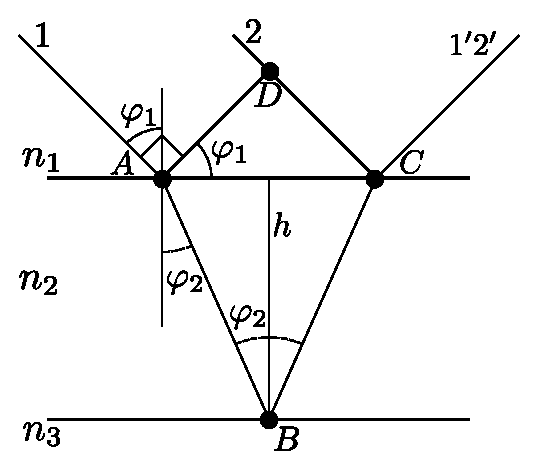
\includegraphics[width=1\linewidth]{img/o-02_2}
	\caption{Схема интерференции в тонких пленках}
	\label{o-02-slim}
\end{wrapfigure}

\textbf{Интерференция в тонких пленках}
Рассмотрим тонкую пленку с показателем преломления $n_2$, на которую падают лучи света из области с показателем преломления $n_1$ и которая покрывает подложку с показателем преломления $n_3$ (см. Рис. \ref{o-02-slim}).

Выделим луч $1$, падающий на верхнюю поверхность пленки в $A$ под углом $\varphi_1$. Часть его отражается, а часть преломляется с углом преломления $\varphi_2$. Этот луч отражается в $B$ (пренебрежем преломленным лучом), приходит в $C$ и вновь преломляется, образуя луч $1'$.

Положим, что в $C$ приходит луч $2$ принадлежащий тому же фронту волны плоской волны $AD$, так что лучи $1$ и $2$ параллельны и их фазы в $A$ и $D$ одинаковы. Рассмотрим отраженную часть луча $2$: $2'$, пренебрегая преломленной. Лучи $1'$ и $2'$ идут совместно и могут интерферировать. Отыщем оптическую разность хода этих лучей.

Первый луч от $A$ проходит дополнительный путь $ABC$ в среде с показателем преломления $n_2$, оптическая длина этого пути равна:
$$
L_1 = \frac{2 n_2 h}{\cos(\varphi_2)} + \left(\frac{\lambda}{2}\right),
\footnote{
	здесь используется утверждение, что при отражении от оптически более плотной среды фаза изменяется на $\pi$ т.е. добавляется путь $\lambda/2$, из этого следует, что слагаемое $\lambda/2$ добавляется при $n_3 > n_2$.
}
$$

Второй луч от точки равных фаз $D$ проходит путь $DC$ в среде $n_1$. Из $AC = 2h\tg\varphi_2$ и закона преломления лучей $n_1\sin\varphi_1 = n_2\sin\varphi_2$ вычислим оптическую длину пути:
$$
L_2 = 2n_1 h \tg\varphi_2\sin\varphi_1 + \left(\frac{\lambda}{2}\right) =
      2n_2 h \sin\varphi_2\tg\varphi_2 + \left(\frac{\lambda}{2}\right),
\footnote{
	слагаемое $\lambda/2$ появляется при $n_2 > n_1$
}
$$ 
Тогда получим оптическую разность хода $\Delta$:
$$
\Delta = L_1 - L_2 = \frac{2n_2 h \left(1-\sin^2\varphi_2\right)}{\cos\varphi_2}
       + \left(\frac{\lambda}{2}\right)
       = 2n_2 h \cos^2\varphi_2 + \left(\frac{\lambda}{2}\right),
\footnote{
	$\lambda/2$ присутствует, если ровно один луч отражается от оптически более плотной среды.
}
$$
Из закона преломления эту формулу можно переписать через угол падения $\varphi_1$:
$$
\Delta = 2h \sqrt{n_2^2 - n_1^2\sin^2\varphi_1} + \left(\frac{\lambda}{2}\right),
$$
Тогда итоговая формула интенсивности примет вид:
$$
I = 2I_0(1 + \cos(k\Delta)) =
    2I_0\left(1 + \cos\left(2hk\sqrt{n_2^2 - n_1^2\sin^2\varphi_1} + (\pi)\right)\right).
$$
Для пространственной когерентности заметим, что интерферируют лучи, расстояние между которыми равно длине $AD$, т.е. условие пространственной когерентности запишется в виде:
$$
2h\tg\varphi_2\cos\varphi_1 < \rho_\text{ког},
$$


\end{document}